\chapter{Matematyczny opis zagadnienia}
\label{cha:model}

% Twierdzenia
\newtheorem{torricelli}{Prawo Torricellego}[chapter]
\newtheorem{pontriagin-max}{Zasada maksimum Pontriagina}[chapter]

Rozważany układ składa się z trzech zbiorników połączonych szeregowo, czy też kaskadowo.
W związku z tym płyn (woda), którym jest napełniony pierwszy zbiornik, przepływa przez otwór o zadanym oporze wypływu do drugiego zbiornika.
Stamtąd znowu wypływa do przez otwór o zadanym oporze do trzeciego zbiornika, skąd przez kolejny taki otwór wypływa do zewnętrznego naczynia.
Stamtąd woda jest pompowana z powrotem do pierwszego zbiornika.
Całość układu jest przedstawiona schematycznie na rys. \ref{fig:zbiorniki}.


\begin{figure}[hpt]
	\centering
	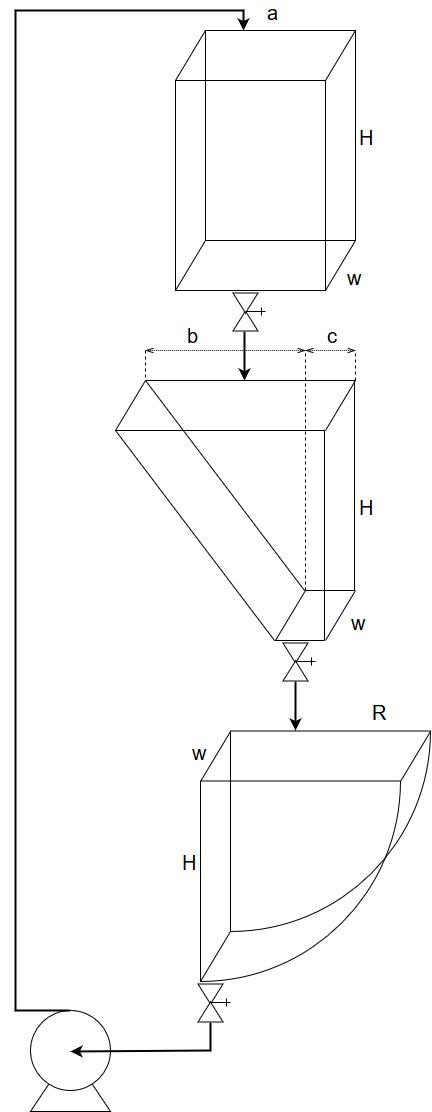
\includegraphics[scale=.5]{Grafika/schemat_zbiornikow}
	\caption{Układ zbiorników z zaznaczonymi wymiarami}\label{fig:zbiorniki}
\end{figure}

\section{Wprowadzenie z zakresu dynamiki płynów}
\label{sec:plyny}

W niniejszym podrozdziale zostały przypomniane podstawowe prawa fizyki związane z przepływem cieczy oraz jego związkiem z poziomem tej cieczy w zbiorniku.

%-------------------------------------------------
\subsection{Równanie Bernoulliego i prawo Torricellego}
\label{sub:plyny-torr}

Równanie Bernoulliego jest jednym z podstawowych praw termodynamiki płynów idealnych. Mówi ono, że wzrost prędkości przepływu cieczy musi wiązać się ze spadkiem ciśnienia lub energii potencjalnej.
Ma kilka postaci; najpopularniejszą jest tzw. szczególne równanie Bernoulliego, które wiąże energię mechaniczną płynu z jego prędkością w danym miejscu, wysokością w układzie odniesienia służącym do wyznaczania energii potencjalnej, ciśnieniem i gęstością.
W takiej formie można je stosować tylko do cieczy nieściśliwych i nielepkich, jednocześnie zakładając stacjonarność i bezwirowość przepływu.

Ta szczególna postać równania Bernoulliego jest przedstawiona jako równanie \ref{eq:bernoulli}.

\begin{equation}\label{eq:bernoulli}
e_{m} = \frac{v^2}{2} + gh + \frac{p}{\rho} = const
\end{equation}

Oznaczenia:
\begin{itemize}
	\item $e_{m}$ - energia jednostki masy cieczy,
	\item $v$ - prędkość cieczy w danym miejscu,
	\item $g$ - przyspieszenie grawitacyjne,
	\item $h$ - wysokość w układzie odniesienia, w którym jest wyznaczana energia potencjalna,
	\item $p$ - ciśnienie cieczy w danym miejscu,
	\item $\rho$ - gęstość cieczy.
\end{itemize}

Z równania Bernoulliego można wyprowadzić bezpośrednią zależność między prędkością cieczy a jej poziomem w zbiorniku. Jest ona znana pod nazwą prawa Torricellego i przedstawiona jako równanie \ref{eq:torricelli} (przyjęto oznaczenia takie jak w przypadku równania \ref{eq:bernoulli}).
Można owo prawo zapisać w bardziej ogólnej formie słownej:

\begin{torricelli}
    Prędkość wypływu cieczy jest proporcjonalna do pierwiastka kwadratowego z poziomu cieczy w zbiorniku.
    \begin{equation}\label{eq:torricelli}
    v = \sqrt{2gh}
    \end{equation}
\end{torricelli}
Takie sformułowanie tego prawa będzie istotne w dalszych krokach wyznaczania modelu matematycznego rozważanego układu.


\subsection{Bilans masy}
\label{sub:plyny-bilans}

Kolejnym zjawiskiem fizycznym, którego zrozumienie jest potrzebne, aby wyznaczyć model matematyczny rozważanego w niniejszej pracy układu zbiorników, jest bilans masy, czyli bezpośrednia konsekwencja \emph{prawa zachowania masy}.

\begin{mass}
    Masa układu ciał (suma mas wszystkich ciał wchodzących w skład tego układu) nie zmienia się podczas przemian i oddziaływań fizycznych w nim zachodzących.
    \begin{equation}\label{eq:mass-conservation}
        m_{uk} = const
    \end{equation}
\end{mass}

Rozważając układ pojedynczego zbiornika z cieczą, do którego ta ciecz jest nalewana i z którego się ona wylewa, można sformułować następstwo tego prawa dane równaniem \ref{eq:mass-balance}. Mówi ono, że zmiana masy w rozważanym zbiorniku - $m_{zb}$ - jest równa zmianie masy do niego wpływającej - $m_{we}$ - i wypływającej - $m_{wy}$.

\begin{equation}\label{eq:mass-balance}
    \frac{\partial m_{we}}{\partial t} - \frac{\partial m_{wy}}{\partial t} =\frac{\partial m_{zb}}{\partial t}
\end{equation}

Przyjmując założenie, że ciecz w zbiorniku i poza nim ma stałą gęstość $\rho$ oraz stosując następujące podstawienia:
\begin{itemize}
    \item $m_{zb} = V_{zb}\cdot\rho$, gdzie $V_{zb}$ to objętość cieczy w zbiorniku,
    \item $V_{zb} = A_{zb} \cdot h_{zb}$, gdzie $A_{zb}$ to pole przekroju poprzecznego zbiornika, a $h_{zb}$ to wysokość słupa cieczy w tym zbiorniku
\end{itemize}
można przedstawić powyższą zależność w postaci opisanej zależnością \ref{eq:tank-mass-balance} (za: \cite{Postlethwaite}).

\begin{equation}\label{eq:tank-mass-balance}
    A_{zb} \cdot \frac{\partial h_{zb}}{\partial t} = \frac{\partial V_{we}}{\partial t} - \frac{\partial V_{wy}}{\partial t}
\end{equation}

Strumień (zmiana objętości cieczy w czasie) wypływający z takiego zbiornika można otrzymać na podstawie prawa Torricellego - jest on dany zależnością \ref{eq:tank-outflow}, gdzie $C$ to stała proporcjonalności wypływu. W rozważanym układzie będzie on zależeć od ustawienia zaworu wyjściowego z danego zbiornika, a więc można powiedzieć, że strumień opisuje opór wypływu ze zbiornika (za: \cite{TanksManual}).

\begin{equation}\label{eq:tank-outflow}
\frac{\partial V_{wy}}{\partial t} = C\cdot\sqrt{h_{zb}}
\end{equation}

Jeśli chodzi o strumień wpływający, to dla drugiego i trzeciego zbiornika jest on równy strumieniowi wypływającemu z poprzedniego zbiornika. Można przyjąć, że dla pierwszego zbiornika ten strumień to sterowanie pompą. Będzie ono oznaczone symbolem $u$.

Pola powierzchni przekrojów poprzecznych wszystkich trzech zbiorników przedstawiono jako równanie \ref{eq:model-fields}. Zastosowano oznaczenia z \ref{fig:zbiorniki}.

\begin{equation}\label{eq:model-fields}
    \begin{array}{lr}
        A_{1} = w \cdot a \\
        A_{2} = c\cdot w + \frac{h_{2}}{h_{max}}\cdot b\cdot w \\
        A_{3} = w\cdot \sqrt{R^{2} - (R - h_{3})^{2}}
    \end{array}
\end{equation}

%-------------------------------------------------
\subsection{Rodzaje przepływów}
\label{sub:plyny-przeplywy}

Przytoczona wcześniej szczególna postać równania Bernoulliego (równanie \ref{eq:bernoulli}) jest obwarowana założeniem stacjonarności przepływu. Oznacza to dwie rzeczy:
\begin{enumerate}
    \item Wartości wektorów prędkości cieczy są stałe w czasie.
    \item Poszczególne ,,warstwy'' cieczy nie wpływają na siebie.
\end{enumerate}

Drugi z tych warunków jest znany pod nazwą przepływu laminarnego, który zwykle ma miejsce przy niskich prędkościach cieczy. W takim typie przepływu nie występują żadne jego zaburzenia (ruchy wirowe, prądy przeciwne itp.), a zachowanie poszczególnych ,,warstw'' cieczy porównać można do tasowania kart: przepływają obok siebie bez wpływania jedna na drugą. Jej cząstki będące blisko powierzchni przemieszczają się po liniach równoległych do tafli cieczy.

Niestety, w rzeczywistości ciężko jest spełnić założenie laminarności przepływu, nie mówiąc już o jego stacjonarności. W związku z tym można zastosować pewne praktyczne uogólnienie zależności \ref{eq:tank-outflow} w stosunku do cieczy wypływających w sposób nielaminarny. Polega ono na zastąpieniu pierwiastka we wspomnianym wzorze parametrem $\alpha$, którego wartość można dobrać na podstawie pomiarów w rzeczywistym układzie (przykład podany w \cite{TanksManual}). Uwzględniają to uogólnienie, można zapisać nowe sformułowanie zależności \ref{eq:tank-outflow} jako równanie \ref{eq:tank-outflow-nonlmnr}.

\begin{equation}\label{eq:tank-outflow-nonlmnr}
    \frac{\partial V_{wy}}{\partial t} = C\cdot h_{zb}^{\alpha}
\end{equation}


\section{Model matematyczny zestawu zbiorników}
\label{sec:model}

Na podstawie podanych wcześniej zależności można zdefiniować model matematyczny rozważanego układu zbiorników.
Jest on dany równaniem \ref{eq:model} (za: \cite{TanksManual}).

\begin{equation}\label{eq:model}
\left \{
\begin{array}{lr}
\frac{\partial h_{1}}{\partial t} = \frac{u - C_{1}{h_{1}}^{\alpha_{1}}}{aw} \\[8pt]
\frac{\partial h_{2}}{\partial t} = \frac{C_{1}{h_{1}}^{\alpha_{1}} -  C_{2}{h_{2}}^{\alpha_{2}}}{cw + \frac{h_{2}}{h_{max}}bw} \\[12pt]
\frac{\partial h_{3}}{\partial t} = \frac{C_{2}{h_{2}}^{\alpha_{2}} -  C_{3}{h_{3}}^{\alpha_{3}}}{w\sqrt{R^{2} - (R - h_{3})^{2}}}
\end{array}
\right.
\end{equation}

Oznaczenia:
\begin{itemize}
    \item $h(t) = [h_{1}(t)~ h_{2}(t)~ h_{3}(t)]^{T}$ - poziomy wody w zbiornikach,
    \item $u(t)$ - sterowanie pompą,
    \item $a$ - szerokość pierwszego zbiornika,
    \item $b$ - szerokość trójkątnej części drugiego zbiornika,
    \item $c$ - szerokość prostopadłościennej części drugiego zbiornika,
    \item $R$ - promień trzeciego zbiornika,
    \item $w$ - głębokość zbiorników,
    \item $h_{max}$ maksymalna wysokość słupa wody w zbiornikach,
    \item $C_{i}$ - opór wypływu z $i$-tego zbiornika,
    \item $\alpha_{i}$ - współczynnik wypływu z $i$-tego zbiornika.
\end{itemize}

Wszystkie wymiary w powyższym wzorze zostały przedstawione na rys. \ref{fig:zbiorniki}. Są na nim również oznaczone opory wypływów $C_{1}$ - $C_{3}$ przy odpowiednich zaworach.

Przyjmując $\alpha_{i} = \frac{1}{2}, \forall_{i \in \{1, 2, 3\}}$, można uszczegółowić powyższy model, zakładając tylko przepływ laminarny.
Taka właśnie jego postać będzie wykorzystywana przy analitycznym wyznaczeniu współczynników równania sprzężonego (definicja znajduje się w sekcji \ref{sub:toc-def-intro}), które jest przeprowadzone w podrozdziale \ref{sub:toc-ctrl}.
W rzeczywistości, jak zostało wspomniane w podrozdziale \ref{sub:plyny-przeplywy}, wartości tych współczynników będą musiały być trochę mniejsze, aby oddać faktyczny sposób przepływu wody między zbiornikami.

W rozważanym układzie zbiorników przyjmuje się następujące ograniczenia (pomijając oczywiste $t \geq 0$):
\begin{itemize}
    \item ograniczenia równościowe:
    \begin{equation}\label{eq:model-eq-const}
    \begin{array}{lr}
        h_{1}(0) = h_{10}\\
        h_{2}(0) = h_{20}\\
        h_{3}(0) = h_{30}\\
    \end{array}
    \end{equation}
    \item ograniczenia nierównościowe:
    \begin{equation}\label{eq:model-noneq-const}
    \begin{array}{lr}
        \forall_{t \in [0, T]}:~ 0 \leq h_{1}(t) \leq h_{max}\\
        \forall_{t \in [0, T]}:~ 0 \leq h_{2}(t) \leq h_{max}\\
        \forall_{t \in [0, T]}:~ 0 \leq h_{3}(t) \leq h_{max}\\
        \forall_{t \in [0, T]}:~ 0 \leq u(t) \leq u_{max}
    \end{array}
    \end{equation}
\end{itemize}
Parametry $h_{10}$, $h_{20}$ i $h_{30}$ oraz $h_{max}$ traktuje się jako zadane.

Punkty równowagi (nazywane również stanami ustalonymi) takiego systemu będą opisane przez zależność \ref{eq:steady-state-def-model} i wyznaczone przez parę wektora wartości zmiennych stanu $h_{r}$ oraz sterowania $u_{r}$. Brak zależności od czasu owej pary został odpowiednio odnotowany.

\begin{equation}\label{eq:steady-state-def-model}
\frac{\partial h(t)}{\partial t} = 0 ~\Rightarrow~ 
\left \{
\begin{array}{lr}
    \frac{\partial h_{1}}{\partial t} = 0 \\
    \frac{\partial h_{2}}{\partial t} = 0 \\
    \frac{\partial h_{3}}{\partial t} = 0
\end{array}
\right.
\end{equation}

Dla rozważanego układu zbiorników będą miały postać daną zależnością \ref{eq:model-steady-state}.

\begin{equation}\label{eq:model-steady-state}
\begin{array}{lr}
u_{r} = C_{1}h_{1}^{\alpha_{1}} = C_{2}h_{2}^{\alpha_{2}} = C_{3}h_{3}^{\alpha_{3}}\\
h_{r} = \begin{bmatrix}
h_{1r}\\h_{2r}\\h_{3r}
\end{bmatrix}
=
\begin{bmatrix}
\big( \frac{\textstyle u_{r}}{\textstyle C_{1}}\big)^{\frac{\scriptstyle 1}{\scriptstyle \alpha_{1}}}\\
\big( \frac{\textstyle u_{r}}{\textstyle C_{2}}\big)^{\frac{\scriptstyle 1}{\scriptstyle \alpha_{2}}}\\
\big( \frac{\textstyle u_{r}}{\textstyle C_{3}}\big)^{\frac{\scriptstyle 1}{\scriptstyle \alpha_{3}}}
\end{bmatrix}
\end{array}
\end{equation}

Wynika z tego, że układ otwarty jest asymptotycznie stabilny, gdyż posiada tylko jeden, zerowy punkt równowagi (pokazany jako wzór \ref{eq:model-zero-state}). Jest to również zgodne z fizyczną naturą tego systemu zbiorników: przy braku zasilania go pompą, cała woda wycieknie ze wszystkich trzech zbiorników.

\begin{equation}\label{eq:model-zero-state}
h_{r}^{0} = \begin{bmatrix}
h_{1r}^{0}\\h_{2r}^{0}\\h_{3r}^{0}
\end{bmatrix} = 
\begin{bmatrix}
0\\0\\0
\end{bmatrix}
\end{equation}


\section{Regulacja czasooptymalna}
\label{sec:toc}

W niniejszym podrozdziale przedstawiona zostanie koncepcja regulacji czasooptymalnej. Zostaną podane założenia zagadnienia, twierdzenia, na których podstawie można wyliczyć rozwiązanie oraz jego proponowana forma analityczna.

Zaznacza się, że mimo iż podane niżej definicje i założenia są wzięte z ogólnych zagadnień optymalizacji dynamicznej, to w podanym brzmieniu stosują się tylko do zagadnienia wyznaczania sterowania czasooptymalnego.

%-------------------------------------------------
\subsection{Ogólna definicja zagadnienia}
\label{sub:toc-def}

%-------------------
\subsubsection{Założenia wstępne}
\label{sub:toc-def-intro}
Przyjmijmy system dany stacjonarnym, zwyczajnym równaniem różniczkowym (pokazanym jako równanie \ref{eq:general_system}), w którym:

\begin{equation}\label{eq:general_system}
    \frac{\partial x(t)}{\partial t} = f(x(t), u(t)), ~ 0 \leq t \leq T
\end{equation}

\begin{itemize}
    \item wektor zmiennych stanu w chwili $t$ - $x(t)$ spełnia następujące założenia:
    \begin{itemize}
        \item $\forall_{t \geq 0}:~ x(t) \in \mathbb{R}^{n}$ - ma $n$ składowych, a więc rozważany system ma $n$ równań różniczkowych zwyczajnych,
        \item $x(0) = x_{0} \in \mathbb{R}^{n}$ - spełnia warunek początkowy $x_{0}$;
    \end{itemize}
    \item wektor sterowań w chwili $t$ - $u(t)$:
    \begin{itemize}
        \item $\forall_{t \geq 0}:~ u(t) \in D \subset \mathbb{R}^{m}$ - ma $m$ składowych zawierającym się w zbiorze $D$ ograniczającym wartości sterowań,
        \item $u(0) = u_{0}$ - spełnia warunek początkowy $u_{0}$,
        \item funkcja $u$ jest przedziałami ciągła na przedziale $[0, T]$, czyli:
        \begin{itemize}
            \item ma co najwyżej skończoną liczbę punktów nieciągłości,
            \item w każdym z nich ma skończoną granicę lewostronną,
            \item jest prawostronnie ciągła,
            \item w lewym końcu przedziału jest lewostronnie ciągła;
        \end{itemize}
    \end{itemize}
    \item funkcja $f: \mathbb{R}^{n} \times \mathbb{R}^{m} \longmapsto \mathbb{R}^{n}$:
    \begin{itemize}
        \item $f \in C^{1}$ - jest ciągła i różniczkowalna ze względu na pierwszy argument,
        \item $\frac{\partial f(t)}{\partial x} \in C^{0}$ - jej pochodna ze względu na pierwszy argument jest ciągła.
    \end{itemize}
\end{itemize}

Rozwiązaniem takiego równania jest oczywiście funkcja $x: [0, T) \longmapsto \mathbb{R}^{n}$ nazywana \emph{trajektorią układu}.

Trajektoria będąca rozwiązaniem zagadnienia minimalnoczasowego musi spełniać następujący warunek końcowy (nazywany również stanem docelowym):
\begin{equation}\label{eq:final_term}
    x(T) = x_{f} \in \mathbb{R}^{n}
\end{equation}

Ów czas $T$, po którym przy danym sterowaniu stan systemu osiągnie warunek końcowy, będzie wskaźnikiem jakości: 
\begin{equation}\label{eq:quality}
    Q(u(t)) = q(x_{f}) = T
\end{equation}

Na tej podstawie można określić \emph{sterowanie optymalne} $\hat{u}(t)$, które spełnia wszystkie wspominane przy opisie równania \ref{eq:general_system} warunki oraz zależność \ref{eq:optimal_quality}. Trajektoria układu wygenerowana przez zastosowanie sterowania optymalnego nazwana jest \emph{trajektorią optymalną} i opisana symbolem $\hat{x}(t)$.
\begin{equation}\label{eq:optimal_quality}
    \forall_{u(t)}:~ Q(u(t)) \leq Q(\hat{u}(t))
\end{equation}

W opisie zagadnienia czasooptymalnego potrzebne są jeszcze dwa pojęcia.
Pierwsze to \emph{funkcja sprzężona} $\psi: [0, T] \longmapsto \mathbb{R}^{n}$ będąca rozwiązaniem tzw. równania sprzężonego \ref{eq:costate-def}.
\begin{equation}\label{eq:costate-def}
\frac{\partial \psi(t)}{\partial t} = - \frac{\partial f(x(t), u(t)}{\partial x}
\end{equation}

Tak, jak w przypadku trajektorii optymalnej układu, trajektoria $\psi(t)$ wyznaczona w układzie, w którym zastosowane zostało sterowanie optymalne $\hat{u}(t)$, nosi nazwę \emph{trajektorii sprzężonej optymalnej} i oznaczona jest symbolem $\hat{\psi}(t)$.

Ostatnim pojęciem potrzebnym w niniejszym zagadnieniu jest \emph{hamiltonian}, zwany również \emph{funkcją Hamiltona}, czyli funkcja $H: \mathbb{R}^{n} \times \mathbb{R}^{n} \times \mathbb{R}^{m} \longmapsto \mathbb{R}$ który dla trajektorii układu $x(t)$ wygenerowanej przy pomocy sterowania $u(t)$ i odpowiadającej im trajektorii sprzężonej $\psi(t)$ zdefiniowany jest zależnością \ref{eq:hamiltonian-def}.

\begin{equation}\label{eq:hamiltonian-def}
H(\psi(t), x(t), u(t)) = \psi(t) \circ f(x(t), u(t)) = \psi(t)^{T} \cdot f(x(t), u(t))
\end{equation}

%-------------------
\subsubsection{Zasada maksimum Pontriagina}
\label{sub:toc-def-pontriagin}

Aby jednoznacznie opisać, a następnie wyznaczyć sterowanie czasooptymalne, potrzebne jest przytoczenie zasadniczego twierdzenia w optymalizacji dynamicznej. Jest ono znane pod nazwą \emph{zasada maksimum Pontriagina}. Zostało opracowane w 1956 r. przez rosyjskiego matematyka Lwa Pontriagina.

\begin{pontriagin-max}\label{the:pontryagin}
    Zakładając układ opisany równaniem \ref{eq:general_system} z warunkiem końcowym \ref{eq:final_term} i wskaźnikiem jakości \ref{eq:quality} oraz równanie sprzężone \ref{eq:costate-def}:\\
    jeśli dla trajektorii układu $\hat{x}(t)$ wygenerowanej przy pomocy sterowania $\hat{u}(t)$ i odpowiadającej im trajektorii sprzężonej $\hat{\psi}(t)$ zachodzi:\\
    \begin{equation}\label{eq:pontriagin}
    \forall_{u(t) \in D}~ \forall_{t \in [0, T]}:~ H(\hat{\psi}(t), \hat{x}(t), \hat{u}(t)) ~ \geq ~ H(\hat{\psi}(t), \hat{x}(t), u(t))
    \end{equation}
    to sterowanie $\hat{u}(t)$ jest sterowaniem optymalnym.
\end{pontriagin-max}

Powyższe twierdzenie należy obwarować dodatkowymi warunkami koniecznymi optymalności. Niech funkcja $g: \mathbb{R}^{2n} \longmapsto \mathbb{R}^{l}$ opisuje zestaw ograniczeń nierównościowych, a funkcja $h: \mathbb{R}^{2n} \longmapsto \mathbb{R}^{k}$ - ograniczeń równościowych. Obie dane są wzorem \ref{eq:pontryagin-constraints}. Dodatkowo zakłada się, że $g, h \in C^{1}$.
\begin{equation}\label{eq:pontryagin-constraints}
    \begin{array}{lr}
    g(x_{0}, x_{f}) \leq 0 \\
    h(x_{0}, x_{f}) = 0
    \end{array}
\end{equation}

Ponadto, zakłada się, że istnieją $\lambda \in \mathbb{R}$, $\mu \in \mathbb{R}^{l}$ oraz $\rho \in \mathbb{R}^{k}$, które wraz z uprzednio zdefiniowanymi wielkościami i funkcjami spełniają następujące \emph{warunki konieczne optymalności}:
\begin{itemize}
    \item warunek nieujemności:
    \begin{equation}\label{eq:pontryagin-noneg}
    \lambda \geq 0 \land \|\mu\| \geq 0
    \end{equation}
    \item warunek nietrywialności:
    \begin{equation}\label{eq:pontryagin-notriv}
    \lambda + \|\mu\| + \|\rho\| > 0
    \end{equation}
    \item warunek komplementarności:
    \begin{equation}\label{eq:pontryagin-comp}
    \mu \circ g(x_{0}, x_{f}) = 0
    \end{equation}
    \item warunki transwersalności:
    \begin{equation}\label{eq:pontryagin-trans}
    \begin{array}{lr}
        \hat{\psi}(0) = \frac{\partial (\mu \circ g + \rho \circ h)}{\partial x_{0}}\\[8pt]
        \hat{\psi}(T) = - \frac{\partial (\mu \circ g + \rho \circ h)}{\partial x_{f}}\\[8pt]
        \forall_{t \in [0, T]}:~ H(\psi(t), x(t), u(t)) = \frac{\partial (\lambda T + \mu \circ g + \rho \circ h)}{\partial T} = \lambda
    \end{array}
    \end{equation}
    \item równanie sprzężone dane wzorem \ref{eq:costate-def},
    \item warunek maksimum hamiltonianu dany wzorem \ref{eq:pontriagin}.
\end{itemize}

%-------------------------------------------------
\subsection{Wyznaczanie sterowania czasooptymalnego}
\label{sub:toc-ctrl}

Analityczne rozwiązania poszukiwania sterowania czasooptymalnego zwykle opierają się bezpośrednio na przytoczonej powyżej zasadzie maksimum i warunkach koniecznych optymalności. W niniejszym podrozdziale zostanie pokrótce przedstawiona droga mogąca zmierzać do wyznaczenia analitycznego czasooptymalnego sterowania w rozważanym układzie zbiorników. Całe rozwiązanie nie jest przeprowadzone ze względu na fakt, iż równiania sprzężone są niestacjonarne, a więc ich rozwiązanie analityczne byłoby bardzo trudne lub wręcz niemożliwe.

Aby dodatkowo uprościć analizę problemu oraz fizyczne zastosowanie wyznaczonego sterowania, zakłada się, że poszukiwane jego postaci będą klasy "bang - bang". To znaczy, że będą przyjmowały tylko wartości z brzegów zbioru dopuszczalnego $D$. Można przyjąć takie założenie, ze względu na to, iż:
\begin{itemize}
    \item sterowanie $u$ jest jednowymiarowe: $D \in \mathbb{R} \Rightarrow D = [0, u_{max}]$,
    \item %TODO: dopisać dlaczego można stosować sterowanie bang-bang
\end{itemize}

Pierwszym krokiem ku wyliczeniu analitycznego rozwiązania jest wyznaczenie równań sprzężonych za pomocą wzoru \ref{eq:costate-def}. Przyjmując współczynniki $\alpha_{i} = \frac{1}{2} \forall_{i \in \{1, 2, 3\}}$ w modelu matematycznym zestawu zbiorników danym równaniem \ref{eq:model}, można wyznaczyć równania sprzężone rozważanego układu. Są one dane wzorem \ref{eq:sprzezone}. Pominięto w nim zależności wszystkich funkcji $\psi$ oraz $h$ od czasu, aby uprościć zapis.

\begin{equation}\label{eq:sprzezone}
	\left \{
	\begin{array}{lr}
		\frac{\partial \psi_{1}}{\partial t} =  \psi_{1}\frac{C_{1}}{2aw\sqrt{h_{1}}} - \psi_{2}\frac{C_{1}}{2\sqrt{h_{1}}(cw + \frac{h_{2}}{h_{max}}bw)} \\[20pt]
		\frac{\partial \psi_{2}}{\partial t} = - \psi_{2}\frac{1}{cw + \frac{h_{2}}{h_{max}}bw}(\frac{b(C_{1}\sqrt{h_{1}} - C_{2}\sqrt{h_{2}})}{ch_{max} + bh_{2}} - \frac{C_{2}}{2\sqrt{h_{2}}}) - \psi_{3}\frac{1}{w\sqrt{h_{3}(2R - h_{3})}} \\[20pt]
		\frac{\partial \psi_{3}}{\partial t} = \psi_{3}\frac{-C_{3}(3R - 2h_{3})}{wh_{3}(2R - h_{3})^{\frac{3}{2}}}
	\end{array}
	\right.
\end{equation}

Następnie trzeba by przedefiniować ograniczenia równościowe (dane wzorem \ref{eq:model-eq-const}) i nierównościowe (\ref{eq:model-noneq-const}) tak, aby spełniały założenia funkcji $g$ i $h$ opisane zależnościami \ref{eq:pontryagin-constraints}.
Korzystając z warunków komplementarności (\ref{eq:pontryagin-comp}) oraz nieujemności (\ref{eq:pontryagin-noneg}), powinno się wyznaczyć składowe wektora $\mu$ oraz założyć pewną postać wektora $\rho$.
%TODO: sprawdzic, czy rzeczywiście nie da się wyznaczyć 

Na podstawie tych danych należałoby wyznaczyć warunki początkowy i końcowy danym wzorem \ref{eq:pontryagin-trans} dla powyższych równań sprzężonych, co pozwoliłoby wyznaczyć analityczne wzory opisujące wszystkie składowe trajektorii sprzężonych systemu.


%-------------------------------------------------
\subsection{Nieliniowość układu a sterowanie czasooptymalne}
\label{sub:toc-nonlnr}


%-------------------------------------------------
\subsection{Numeryczne metody wyznaczania sterowania czasooptymalnego}
\label{sub:toc-num}

\section{Regulacja liniowo - kwadratowa}
\label{sec:lqr}

W niniejszym podrozdziale zostanie przedstawione zagadnienie szukania sterowania w układach liniowych z tzw. liniowo-kwadratowym wskaźnikiem jakości. Pokazana zostanie również metoda zastosowania takiego typu regulacji dla układów nieliniowych przy użyciu linearyzacji w punkcie pracy.

%-------------------------------------------------
\subsection{Ogólna definicja zagadnienia}
\label{sub:lqr-def}


%-------------------------------------------------
\subsection{Linearyzacja modelu}
\label{sub:lqr-lin}


%-------------------------------------------------
\subsection{Wyznaczanie regulatora liniowo - kwadratowego}
\label{sub:lqr-ctrl}


%-------------------------------------------------
\subsection{Dobór wag w zagadnieniu liniowo - kwadratowym}
\label{sub:lqr-weights}
